%\documentclass[twocolumn]{scrartcl}
\documentclass[DIV=14,twocolumn]{scrartcl}
\usepackage[pdftex]{hyperref}
\usepackage{cite}
\usepackage{amsmath}
\usepackage{amssymb}
\usepackage[]{algorithm2e}
\usepackage{graphicx}

\DeclareMathOperator{\rank}{rank}
\newcommand{\norm}[1]{\left\lVert#1\right\rVert}

%opening
\title{Statistical learning theory (lab) final project report}
\subtitle{Building a recommender system with matrix factorization}
\author{Markus Fischer\\ \small{\href{mailto:markus.fischer@uni-jena.de}{markus.fischer@uni-jena.de}}}
\date{25.07.2019}

\begin{document}

\maketitle
\begin{abstract}
In times of e-commerce it is useful to predict ratings that  users might give for an item, to recommend them new, unseen items. In the following report I describe on method to do this. I introduce basic metrics and three simple baseline models. Later I give details to the matrix factorization technique. In the final section I show some insights for the parameter tuning of such models.
\end{abstract}

\section{Task and Dataset}\label{intro}
As final project for the course "Statistical Learning Theory (Lab)" we were required to write a recommender system. There are two ways to interpret this task.
The first, less technical interpretation is the following: Roughly speaking, we want to predict the rating $\hat{r}_{u,i}$, that some user $u$ might give to an item $i$, depending on the previous ratings of this user or item.

From a more technical point of view, the task is to complete a highly sparse matrix. The original ratings are composed in a matrix $R\in\mathbb{R}^{m\times n}$, where the rows represent the $m$ users and the $n$ columns the items.
Each entry $r_{u,i}$ then stands for the rating of user $u$ for item $i$. We now want compute a dense matrix $\hat{R}$ were we assign a rating for each user-item pair.

There are many approaches to do this. In \cite{KoBeVo09} two of the most common algorithms for this task are described.
One approach follows the assumption that similar users would rate items similarly. Such algorithms try to determine the distance between two users or items and then use a $k$-Nearest-Neighbor algorithm to compute the rating depending on their ratings.

The second common approach is often called latent factor model. The idea is the following: each item belongs to certain concepts. Each user may like some of these concepts more than others. In the world of films that could be the genre of the movie. A latent factor approach now tries to explain the ratings of items with respect to this categories. Usually they compute a decomposition of the ratings matrix.

\subsection{Dataset Insights}\label{datsetinsight}
We got a set of 461,806 triples in the form (row, column, rating) and we were required to rate another 81,495 row-column pairs. 
The given training data stretches out to a matrix of the dimension $5499\times 2080$. Since this matrix has 11,437,920 possible entries we have around $95.9\%$ sparsity.

Our ratings are in the set $\{0,1,2,3,4\}$. Since 0 is a possible rating, it is useful to apply a feature map $$\phi:\mathbb{N}\rightarrow\mathbb{N},m\rightarrow m+1$$ before any other computation. As a result, we can set empty entries in our ratings matrix to 0. To get our final, correct ratings we should apply the inverse feature map $\phi^{-1}$ as final step.

\subsection{Item and User Bias}\label{bias}
Let us look a bit deeper in our dataset. It is interesting to see how the number of ratings for items is distributed. As shown in \autoref{fig:itemcount}, around one half of the items were rated by users. Most of the rated items received at least 300 ratings. 
\begin{figure}[h]
	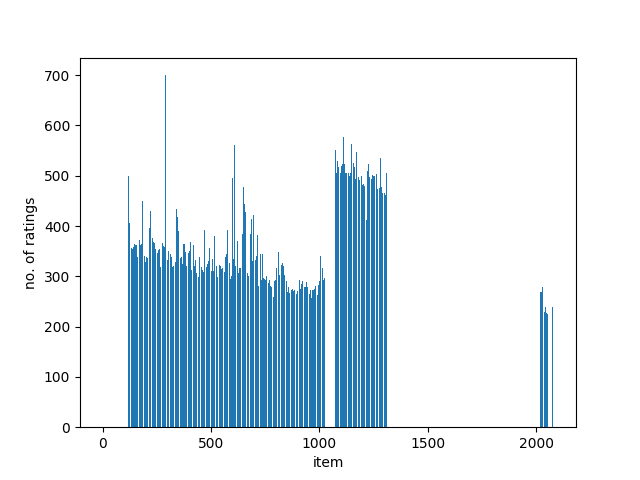
\includegraphics[width=\columnwidth]{../img/item-count}
	\caption{rating count per item}
	\label{fig:itemcount}
\end{figure}

More interesting is the distribution of ratings per user. Looking on \autoref{fig:usercount}, shows that there exist some users that rate around one half of the items. On the other hand, a majority of users rate only a few items. It is therefore safe to assume that the ratings of our users are biased. As a consequence, it is useful to incorporate this bias in the models to improve the prediction.
Since some of the items are also rated more often, there exist a item bias as well, which should be incorporated.
\begin{figure}
	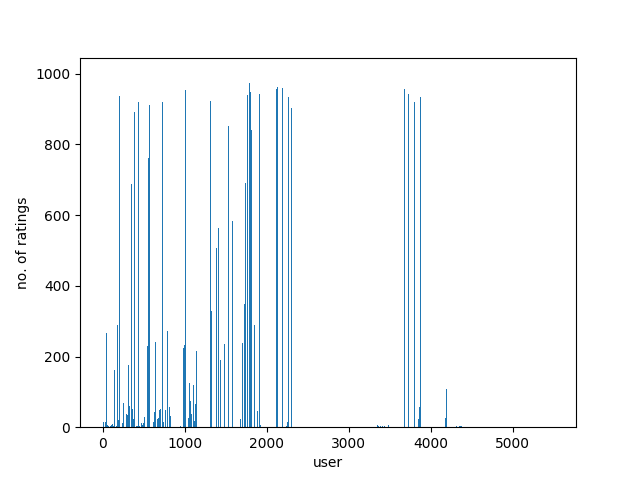
\includegraphics[width=\columnwidth]{../img/user-count}
	\caption{rating count per user}
	\label{fig:usercount}
\end{figure}

\section{Measuring the Performance}
To compare variants of models and for selecting the best one, it is necessary to have a objective measure. There are many different metrics for this. It depends on the concrete task which one we should consider. In this case only the accuracy of the system is necessary. Other interesting metrics could be the coverage of the items, the novelty or the diversity of recommendations.

One common metric to measure the accuracy of a predictor is the root mean square error (RMSE). Let $r_{u,i}$ be the observed rating, $\hat{r}_{u,i}$ the predicted rating and let $n$ be the number of predictions. Then the RMSE is defined in the following way: 
\begin{equation*}
\begin{split}
\text{RMSE} = \sqrt{\frac{\sum_{\text{predicted ratings}} (r_{u,i}-\hat{r}_{u,i})^2}{n}}
\end{split}
\end{equation*}
This is a measure to determine how good a trained model fits on the given dataset. Keep in mind that this metric tends to disproportionately penalize large errors. 


For better results it is common to use only parts of the data set for training. The remaining parts are then used for validation. The advantage of this technique is that we are able to determine overfitting of an estimator. Worse results on the new, unseen validation set, compared to the results of the training set, indicate that the estimator memorizes the training set too well and that it is not able to generalize. This technique is often called cross validation. 

For more metrics and a deeper discussion of predictor validation refer to \cite{Ag16}.

\section{Baseline Predictors}\label{baseline}
To get a feeling of the dataset it is useful to implement very basic baseline predictors. For example it is possible to use the mean of the ratings specified by user $u$ to specify a new rating $\hat{r}_{u,i}$ for item $i$. In an analogue way the mean of an item $i$ could be used as well. A third option is the usage of random values. 

\begin{table}[h]
	\centering
	\begin{tabular}{r|l}
		method & RMSE \\ \hline
		user mean & 0.700 \\
		item mean & 0.772 \\
		random & 1.780
	\end{tabular}
	\caption{RMSE for baseline models}
	\label{tab:baseline}
\end{table}

Splitting our given dataset in a training set and in a test set and using the above described methods gives us the results shown in \autoref{tab:baseline}. The value for the random method was determined after one run. Repeating this experiment would give other values.

The mean methods already give quite good results. The better result of the user mean model can be explained with the bias described in \autoref{bias}. Models that are above these values can be easily ignored. 


\section{Matrix Factorization}\label{matrixfactorization}
A better way to solve such a task is the usage of matrix factorization techniques. The idea is the following: given is a ratings matrix $R\in\mathbb{R}^{m\times n}$. We assume that $\rank(R)=k\ll\min(m,n)$. Then this matrix can be decomposed in two smaller matrices such that 
$$R\approx UV^T$$ holds, where $U\in\mathbb{R}^{m\times k}$ and $V\in\mathbb{R}^{n\times k}$. This is an example for matrix factorization as described in \autoref{intro}. $k$ stands for the number of latent features that should be considered by the model. 

As stated in \cite{KoBeVo09}, one common way to do thi, is the usage of singular value decomposition (SVD), which works fine with dense matrices. In this case the matrix $R$ is highly sparse and SVD wouldn't work. Instead the problem can be reformulated as optimization problem, as described in \cite{Ag16}. The following objective function can be used: 
$$\min_{U,V} \frac{1}{2}\norm{R-UV^T}^2$$ 
$\norm{\cdot}^2$ refers here to the squared Frobenius norm which is defined as $$\norm{A}^2:=\sum_{i,j}A_{i,j}^2.$$

In the easiest variant of such an optimization problem, we assume that there are no further constraints. This variant is therefore called unconstrained matrix factorization (UMF). 
It is common to compute the solution of this problem with the gradient descent method.

\subsection{Gradient Descent}\label{gd}
The gradient descent method is an iterative approach to find an $x$ which minimizes a differentiable function $f$, starting with a given $x^{(0)}$. As a first step it is necessary to compute the gradient $\nabla f$ of the function, which points in the direction of the highest ascent. 
To minimize the function, the idea is now to go small steps in the opposite direction. An algorithm for this is described in \autoref{algo:gd}. 

\begin{algorithm}
	\caption{gradient descent}
	\label{algo:gd}
	\KwData{starting point $x^0$, learning rate $\eta > 0$}
	\KwResult{$x$ that minimizes $f$}

	\While{no convergence}{
		calculate $\nabla f$\;
		update $x^{(n+1)} \leftarrow x^{(n)} - \eta \nabla f$ \;
	}
\end{algorithm}
Note that this is only the easiest example for gradient descent methods. Keep in mind that for a to large $\eta$ the algorithm shows divergence.
For a more detailed description refer to \cite{ShSh14}. 

\subsection{Applying Gradient Descent on UMF} 
We want to apply the gradient descent approach to the unconstrained matrix factorization problem. 
As a first step it is necessary to calculate the gradient of our objective function. 

Since there are only a few observed entries in the ratings matrix $R$, the objective function is undefined. To fix this, it is necessary to set the unobserved entries in $UV^T$ and $R$ to zero. This works only if the feature map $\phi$ given in \autoref{datsetinsight} was applied before. 

Now let us define $E:=R-UV^T$ as the error matrix. Again all unobserved entries in this matrix are zero, and don't affect the loss function. The objective function becomes now \[\min\frac{1}{2}\norm{E}^2.\]
With this in mind, it is possible to calculate the gradient of the objective function.
Let us start with respect to an entry in matrix U.
\begin{equation*}
\begin{split}
\nabla_{U_{i,\beta}} \frac{1}{2}\norm{E}^2 &= \nabla_{U_{i,\beta}} \frac{1}{2}\sum_{i,j}E_{i,j}^2 \\ &=\nabla_{U_{i,\beta}} \frac{1}{2}\sum_{i,j}(R_{i,j}-(UV^T)_{i,j})^2 \\
&=\nabla_{U_{\alpha,\beta}} \frac{1}{2}\sum_{i,j}(R_{i,j}-\sum_{l=1}^k U_{i,l}V^T_{l,j})^2\\
&=\sum_{i,j}(R_{i,j}-\sum_{l=1}^k U_{i,l}V^T_{l,j})(-V^T_{\beta,j})\\
&=\sum_{i,j}(E_{i,j})(-V_{j,\beta})=-EV_{i,\beta}.
\end{split}
\end{equation*}
It is possible to derive the gradient for an entry in matrix V symmetrical. We get 
\begin{equation*}
\begin{split}
\nabla_{V_{j,\alpha}} \frac{1}{2}\norm{E}^2 &= \nabla_{V_{j,\alpha}} \frac{1}{2}\sum_{i,j}(R_{i,j}-(UV^T)_{i,j})^2\\
&=\sum_{i,j}(E_{i,j})(-U_{i,\alpha})=-E^TU_{j,\alpha}.
\end{split}
\end{equation*}
Those gradients can be easily vectorized to $\nabla_U \frac{1}{2}\norm{E}^2=-EV$ and  $\nabla_V \frac{1}{2}\norm{E}^2=-E^TU.$ Since the learning rate $\eta$ needs to be positive we get the following update rules: \[U^{(i+1)} \leftarrow U^{(i)} + \eta E^{(i)}V^{(i)}\] \[V^{(i+1)} \leftarrow V^{(i)} + \eta E^{(i)T}U^{(i)}.\]
For minimizing the objective function with \autoref{algo:gd}, it is necessary to have a starting point. One option to obtain $U^{(0)}$ and $V^{(0)}$ is the initialization with random values. 

It is necessary to have convergence criteria or \autoref{algo:gd} would run into a infinite loop. One possibility is that the value of the objective function should be below a certain value. But since the gradient descent finds a local, previously unknown, minimum it is hard to decide when to stop. It is therefore better to use other criteria. 

In my implementation I stop when the difference of the objective function value between two iterations is below a certain limit. Formally the algorithm stops when
\begin{equation*}
\begin{split}
&\left|\frac{1}{2}\norm{E^{(n)}}^2-\frac{1}{2}\norm{E^{(n+1)}}^2\right| =\\
&\frac{1}{2} \left| \sum_{i,j}(E_{i,j}^{(n)})^2-(E_{i,j}^{(n+1)})^2 \right| \leq\epsilon
\end{split}
\end{equation*} $$$$ holds.

It is also common to stop after a certain number of iterations even when we not reached convergence.

\textit{Note:} It is also possible to reshape the matrices into vectors of the dimension $(mk)\times1$ and $(nk)\times1$. This doesn't change the algorithm itself but makes it possible to use more advanced techniques, like the one described in \autoref{improvinggd}.

\subsection{Regularization to Prevent Overfitting}
In order to prevent overfitting, it is common to add a regularization term to the objective function. As stated in \cite{Gi19} this may increase the bias but it also may decrease the variance of the estimator. This is known as bias-variance trade-off and can lead to a better predictor. 

For our matrix factorization problem, it is possible to add the regularization terms $\frac{\lambda}{2}\norm{U}^2$ and $\frac{\lambda}{2}\norm{V}^2$ for $\lambda \geq 0$ as recommended in \cite{Ag16}.
Plugging this into the objective function lead to the following problem: $$\min_{U,V} \frac{1}{2}\norm{E}^2 + \frac{\lambda}{2}\norm{U}^2 + \frac{\lambda}{2}\norm{V}^2.$$ Calculating the gradient of this objective function gives two, slightly modified update rules: \[U^{(i+1)} \leftarrow U^{(i)} + \eta E^{(i)}V^{(i)} - \eta\lambda U^{(i)}\] \[V^{(i+1)} \leftarrow V^{(i)} + \eta E^{(i)T}U^{(i)} - \eta\lambda V^{(i)}.\]
Setting $\lambda = 0$ gives the original problem with no regularization. It is therefore possible to use these update rules even in the unregularized case.

\subsection{Incorporating Bias}
Users and items are different. Some users may rate many items and others only a few. And some items are bought more often then others and therefore may have more ratings. We have seen this problem in \autoref{datsetinsight}.
 
A first step to encounter this problem, is to mean center the original matrix with the global mean $\mu$. After this is done, it is necessary to add the mean after calculating the final ratings.

As described in \cite{Ag16} it is possible to improve this approach further. Let us associate with each user $i$ a variable $o_i$, which indicates the bias of user $i$ to rate items. Users who rate items high or more often, might have a high value, users who very rarely rated items may have small (negative) values. Vice versa we can introduce a similar variable $p_j$ for items.
 
The predicted rating now becomes $$\hat{R}_{u,i} = \mu + o_u + p_i + UV^T_{u,i}.$$ Therefore the error matrix can now be written as $$E_{u,i} = R_{u,i}^{'} - \hat{R}_{u,i} = R_{u,i}^{'} - o_u - p_i - UV^T_{u,i}.$$ Note that $R^{'}$ denotes the mean centered data matrix and as a result $\mu$ plays no role in the following calculations.

Now let us look at the following equation:
\begin{equation*}
\begin{split}
o_u + p_i + UV^T_{u,i} &= \sum_{l}^{k}U_{u,l}V^T_{l,i} + o_u + p_i\\ &= \sum_{l}^{k}U_{u,l}V^T_{l,i} + o_u\cdot 1 + 1\cdot p_i.
\end{split}
\end{equation*}
It is easy to see that the last two terms can added to the sum if we increase $k$ by $2$ and set $U_{u,k+1}=o_u$ and $V^T_{k+1,i}=1$ as well $V^T_{k+2,i}=p_i$ and $U_{u,k+2}=1$. The new problem is now similar to our original problem. The only difference is that there are two new small constraints. The column $k+2$ in $U$ and the column $k+1$ in $V$ must be $1$.
On way to satisfy these constraints is the reset to 1 after each iteration of the algorithm as described in \cite{Ag16}.

\subsection{Improving the Gradient Descent}\label{improvinggd}
We have seen that the gradient descent is one method to minimize our optimization problem. But as described in \autoref{gd}, the \autoref{algo:gd} diverges for to large values of $\eta$.
On the other hand for to small $\eta$ the algorithm needs many cycles in order to converge. Therefore the algorithm gives us room for improvements.

One common way is the usage of stochastic gradient descent (SGD). In this case not the gradient of our objective function is used, but a random vector which expectation lies in the subgradient of the function. For a detailed description refer to \cite{ShSh14}.

It is also possible to modify the step size in the algorithm itself. The idea is to choose $\eta$ in a way that it should be large enough to minimize the function fast, but small enough to show no divergence. 

The best $\eta$ would be the one, that minimizes $$\psi(\eta) = f(x-\eta\nabla f(x))$$ for $\eta > 0$. The brute-force algorithm would perform a linear search on $\eta$. But this is computationally expensive.  But there exist multiple numerical methods, to find such $\eta$ in fast time. For example such $\eta$ could meet the Wolfe conditions, as described in \cite{NoWr06}:
\begin{equation*}
\begin{split}
f(x-\eta\nabla f(x)) \leq f(x) + c_1\eta\nabla f^T\nabla f(x)
\end{split}
\end{equation*}
\begin{equation*}
\begin{split}
\nabla f(x-\eta\nabla f(x))^T\nabla f(x) \geq c_2\nabla f^T\nabla f(x)
\end{split}
\end{equation*}
for $0 < c_1 < c_2 < 1$.
Algorithms using this for an modified line search converge much faster than the brute-force algorithm.

Incoporating this into \autoref{algo:gd}, the computation of $\eta$ now needs more time, but since the step size now fits better, we need less cycles and therefore our algorithm should converge faster. 

Note the following: Since $\eta$ is not fixed it is not certain that $$\left|\frac{1}{2}\norm{E^{(n)}}^2-\frac{1}{2}\norm{E^{(n+1)}}^2\right|$$ becomes smaller in each iteration. Sometimes the improved algorithm makes big steps. But our convergence criteria work, since the steps will get asymptotically smaller. Also the objective function value becomes smaller from iteration to iteration, and so the algorithm is correct. 

Keep also in mind that there is a chance that the modified line search algorithm does not converge, since it is a numerical approach. There are two options to handle this problem. In this case it is possible to set $\eta$ to a small value and hope that it converges in the next iteration. The other option is simply to stop the algorithm in this case.

\section{Model Evaluation And Parameter Tuning}\label{parametertuning}
The model described in \autoref{matrixfactorization} has two main parameters. The most important one is the rank of the decomposition matrices. The second interesting parameter is the regularization parameter $\lambda$. It would also be interesting to see the impact of the bias variables.

For the following experiment the given data set was split in two halves. 90\% of the data set were used for training. The remaining 10\% were used to calculate the RMSE. 

The matrix rank has more impact on the result, because it determines how many latent factors the model should consider for ratings. It is therefore useful to start the search there. I trained 5 models with ranks 1 to 20 in steps of five. I used constant $\eta=0.0005$, no regularization and the convergence criteria $\varepsilon = 0.001$. The maximum cycle count was set to 5000. To see an impact of the bias variables, I repeated the experiment with the same learning parameters but incorporating bias variables.  
\begin{figure}[h]
	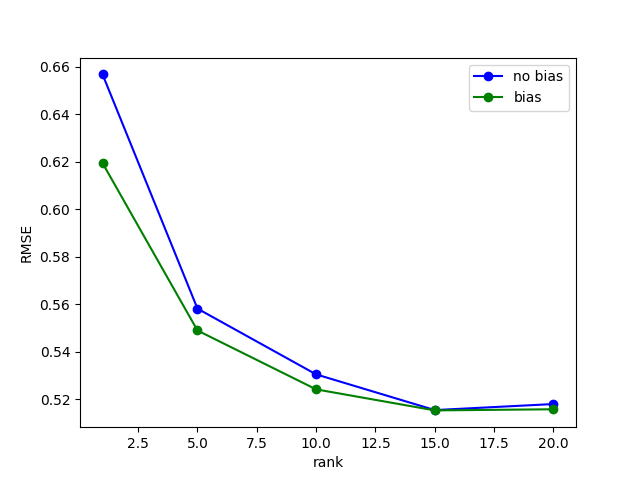
\includegraphics[width=\columnwidth]{../img/rank-rmse-validate}
	\caption{RMSE vs. matrix rank}
	\label{fig:ranksearch}
\end{figure}
The result of these experiments are shown in \autoref{fig:ranksearch}. Compared to our baseline models of \autoref{baseline}, even the model with rank 1 performs better. The performance of our models increase til rank 15. It is noticeable that the performance increases, but decreases for larger ranks.
Between rank 15 and rank 20 the unbiased estimator performance gets worse again. This might be a sign for overfitting. The other possible explanation is that every model comprises some randomness for the starting point. 
 
If we look at the biased estimator it is clearly visible that the incorporation of bias variables has a huge impact on low rank models. With increasing rank the influence of the bias variables vanishes. At rank 15 they have nearly no impact. 
This is no surprise. The two extra variables virtually increase the rank of the matrix, so the results should be better.
But on the other hand, it seems that biased estimators tend to overfit less.

It is also interesting to see, that a model which uses only the bias variables can give good results too. The bias variables seem useful and it makes sense to incorporate them in the final model.
\begin{figure}[h]
	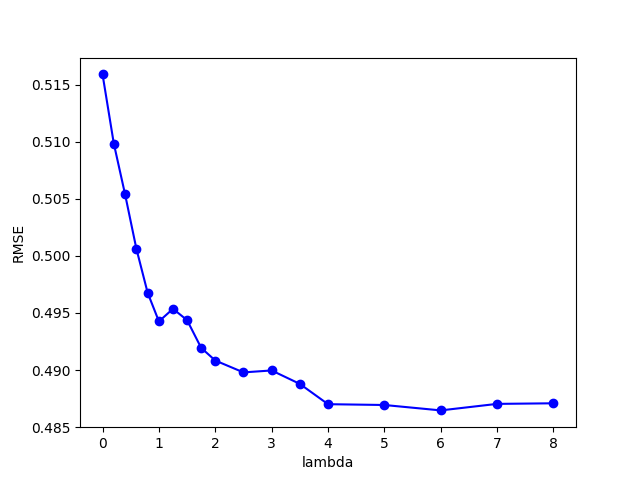
\includegraphics[width=\columnwidth]{../img/lambda-rmse-validate}
	\caption{RMSE vs. regularization parameter $\lambda$}
	\label{fig:lambdasearch}
\end{figure}

The last parameter that has direct impact on the performance, is the regularization parameter $\lambda$. To determine the optimal $\lambda$ I choose the biased model with rank 20 from the previous experiment, as it is the best performing model without regularization. Learning rate and maximum cycle count were also the same values as above. 
I decided to test values for $\lambda$ between 0 and 8. From 0 to 1 I used a step size of 0.2, from 1 to 2 a step size of 0.25 and from 2 to 4 a step size of 0.5. The step size for the last models was set to 1. As shown in \autoref{fig:lambdasearch} the regularization has a huge impact up to  $\lambda=1$. The performance continues to rise until $\lambda=4$. From this point on, there isn't any noticeable performance boost using a higher value for this parameter. 
The variation between some iterations should come from the random starting point for our model training. 
\section{Conclusion}
With the results of the parameter tuning, as described in \autoref{parametertuning}, I trained a final model with rank 19 and $\lambda=4$ with adaptive step size for the improved gradient descent out of \autoref{improvinggd}. I originally wanted to use rank 20, but for this, the line search did not converge. 
Using this configuration gave a final result of 0.617 on the evaluation platform. Note that training the model with the same parameters again might lead to different results, because of the randomness involved. The final code can be found under \url{https://github.com/MarkusFischer/sll-recommender}. 

The result is good but not perfect. Other techniques might give better results. Here we have only positive ratings. So we could constraint our matrix factorization to be not negative. Such variants are called non-negative matrix factorization (NMF).

On the other hand it would be interesting to see how $k$-Nearest-Neighbor methods perform. I tried to implement such approach but got pretty bad results. With more time it would be interesting to see how a combination of both methods perform.

\bibliography{references}{}
\bibliographystyle{alpha}
\end{document}
